% !TeX root = ../defense.tex

\section{Background Information}
\frame{\sectionpage}

\begin{frame}{Databases}
    \begin{alertblock}{How do databases store, retrieve and manipulate data?}
        \begin{enumerate}[<+->]
            \item Where is the data stored? Centralised, Distributed, Personal
            \item Is the data format fixed? SQL vs NoSQL
            \item What are the requirements? Scale, operations to be performed, QoS metrics to meet.
            \item What operations are going to be performed? E.g. Updates, Deletes, adding new fields, queries to be answered
            \item Online system or offline system? Handling static data Vs Data streams.
        \end{enumerate}
    \end{alertblock}
\end{frame}

\begin{frame}{SQL Vs NoSQL}
    \begin{alertblock}{Some of the differences between these two are:-}
        \begin{enumerate}[<+->]
            \item SQL databases are table based databases whereas NoSQL databases can be document based, key-value pairs, graph databases.
            \item SQL databases are vertically scalable while NoSQL databases are horizontally scalable.
            \item SQL databases have a predefined schema whereas NoSQL databases use dynamic schema for unstructured data.
            \item SQL requires specialized DB hardware for better performance while NoSQL uses commodity hardware.
            \item SQL is an ideal choice for the complex query intensive environment and NoSQL is a best used for solving data availability problems. 
        \end{enumerate}
    \end{alertblock}
\end{frame}

\begin{frame}{SQL}
    In the thesis we focus on Structured Query Language.\\
    How does a SQL database look like?\\
    An SQL database is a collection of tables of data.
    \begin{figure}
        \centering
        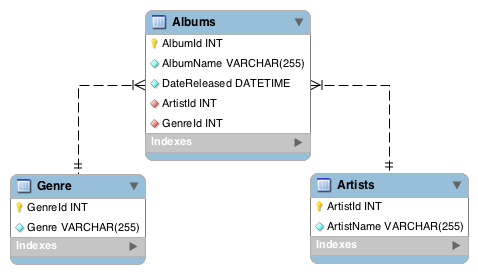
\includegraphics[scale=0.5]{db_example.png}\\
        \caption{Album database}
        \label{fig:db_ex}
    \end{figure}
\end{frame}
    
\begin{frame}{SQL}
    How does a table in SQL look like?\\
    A table can be thought of a matrix, with each row representing a data point and column representing the attribute value for the data point.
    \begin{figure}
        \centering
        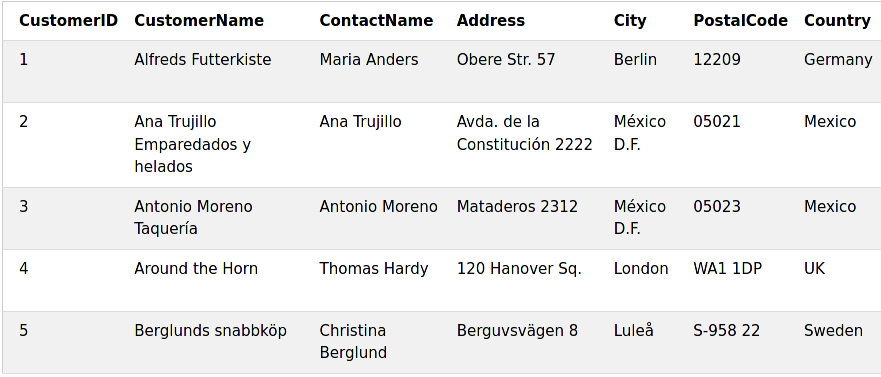
\includegraphics[scale=0.35]{table_example.png}\\
        \caption{Customer Database}
        \label{fig:table_ex}
    \end{figure}
\end{frame}

\begin{frame}[fragile]{SQL}
    What is a SQL query? \\
    An SQL query is a question or a request for answer on a database.
    \begin{lstlisting}[language=SQL,caption=SQL statement selects all the customers from the country "Mexico" in the "Customers" table, label={lst:sql_ex}]
        SELECT * FROM Customers
        WHERE Country='Mexico';
    \end{lstlisting}
\end{frame}

\begin{frame}[fragile]{SQL}
    Hows is a SQL query executed?
    \begin{lstlisting}[language=SQL, caption= SQL query to convert]
        SELECT MovieTitle
        FROM StarsIn
        WHERE StarName IN(
            SELECT name
            FROM MovieStar
            WHERE birthdate LIKE '%1960'
        );
    \end{lstlisting}
\end{frame}

\begin{frame}{SQL: Pipeline}
    \begin{figure}
        \centering
        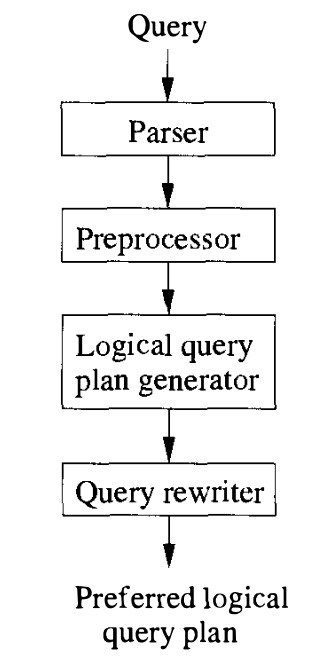
\includegraphics[scale=0.25]{query_processor.png}\\
        \caption{The pipeline for query processing}
        \label{fig:query_processor}
    \end{figure}
\end{frame}

\begin{frame}{SQL: Parser}
    \begin{figure}
        \centering
        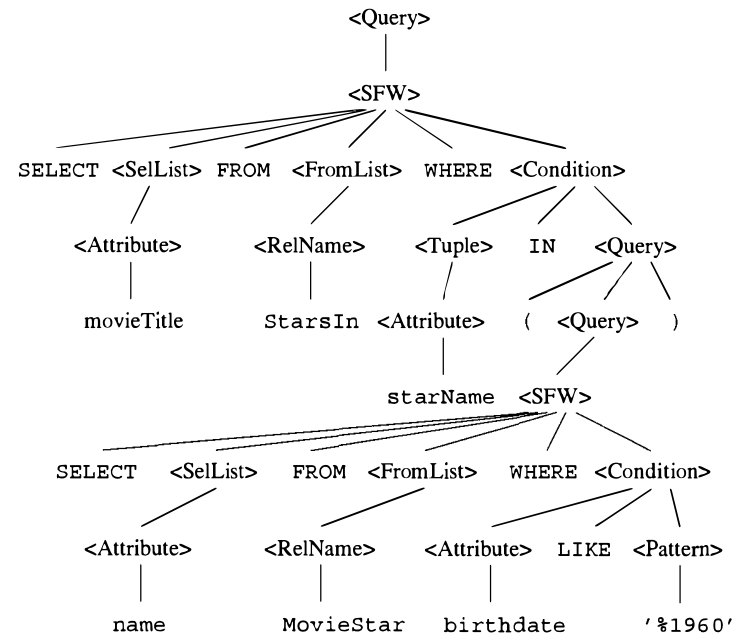
\includegraphics[scale=0.25]{parse_tree.png}\\
        \caption{An example of parse tree}
        \label{fig:prase_tree}
    \end{figure}
\end{frame}

\begin{frame}{SQL: Relational Algebra: Selection}
    \begin{figure}
        \centering
        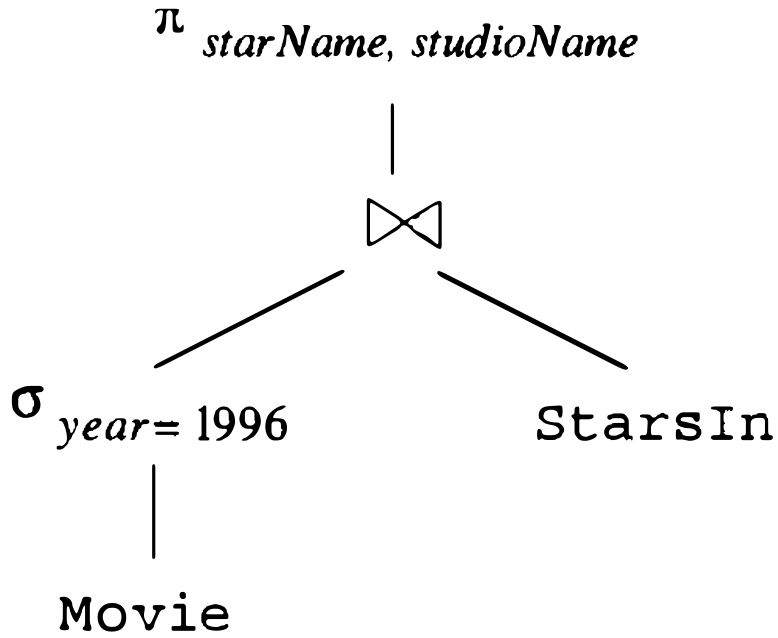
\includegraphics[scale=0.25]{selection_pushdown1.png}\\
        \caption{An example of selection being pushed down for optimization}
        \label{fig:s_p_1}
    \end{figure}
\end{frame}

\begin{frame}{SQL: Relational Algebra: Selection}
    \begin{figure}
        \centering
        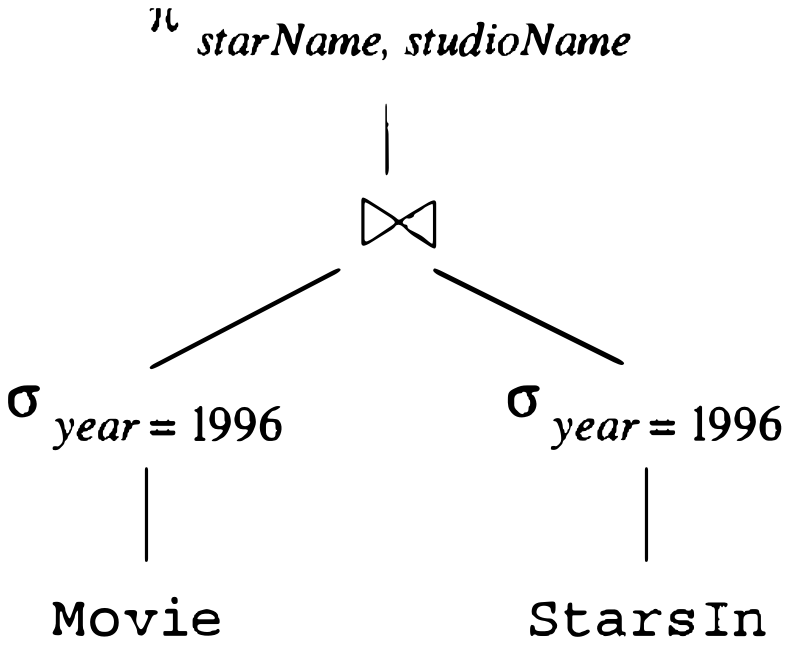
\includegraphics[scale=0.25]{selection_pushdown2.png}\\
        \caption{An example of selection being pushed down for optimization}
        \label{fig:s_p_2}
    \end{figure}
\end{frame}

\begin{frame}{SQL: Relational Algebra: Projection}
    \begin{figure}
        \centering
        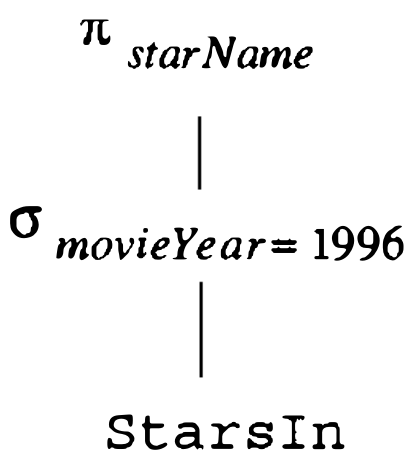
\includegraphics[scale=0.25]{projection_pushdown1.png}\\
        \caption{An example of projection being pushed down for optimization}
        \label{fig:p_p_1}
    \end{figure}
\end{frame}

\begin{frame}{SQL: Relational Algebra: Projection}
    \begin{figure}
        \centering
        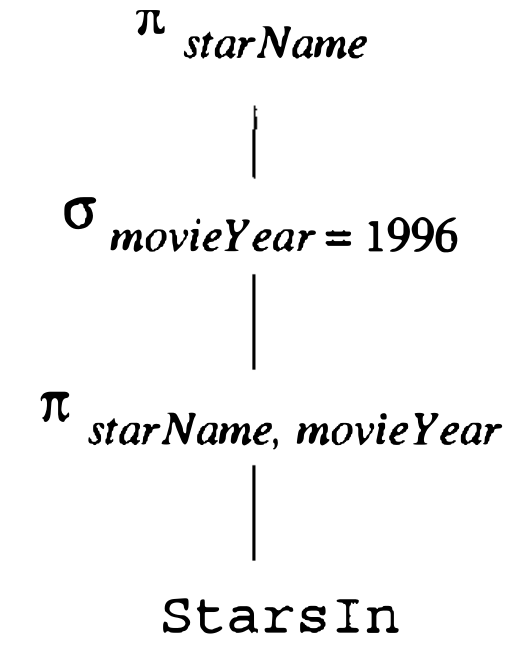
\includegraphics[scale=0.25]{projection_pushdown2.png}\\
        \caption{An example of projection being pushed down for optimization}
        \label{fig:p_p_2}
    \end{figure}
\end{frame}

\begin{frame}{SQL: Relational Algebra: Join}
    \begin{figure}
        \centering
        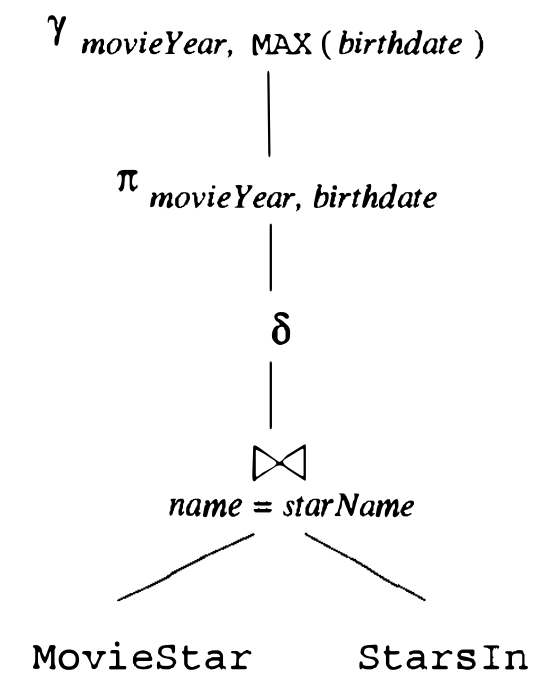
\includegraphics[scale=0.25]{join_pushdown1.png}\\
        \caption{An example of join being optimized}
        \label{fig:j_1}
    \end{figure}
\end{frame}

\begin{frame}{SQL: Relational Algebra: Join}
    \begin{figure}
        \centering
        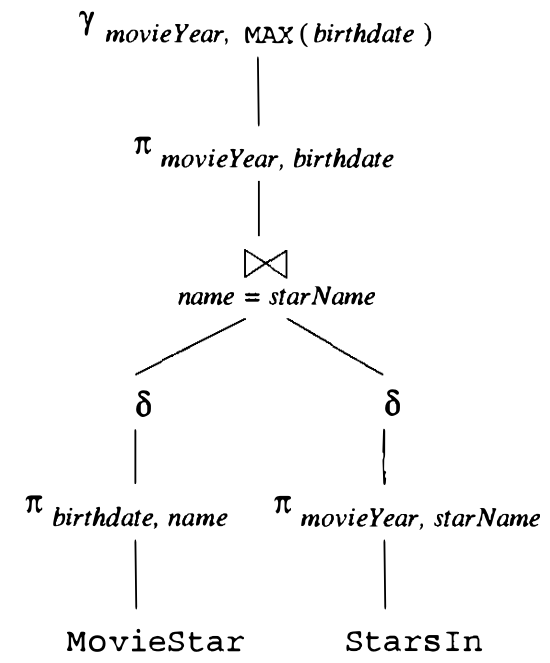
\includegraphics[scale=0.25]{join_pushdown2.png}\\
        \caption{An example of join being optimized}
        \label{fig:j_2}
    \end{figure}
\end{frame}

\begin{frame}{SQL: Grouping operators}
    \begin{figure}
        \centering
        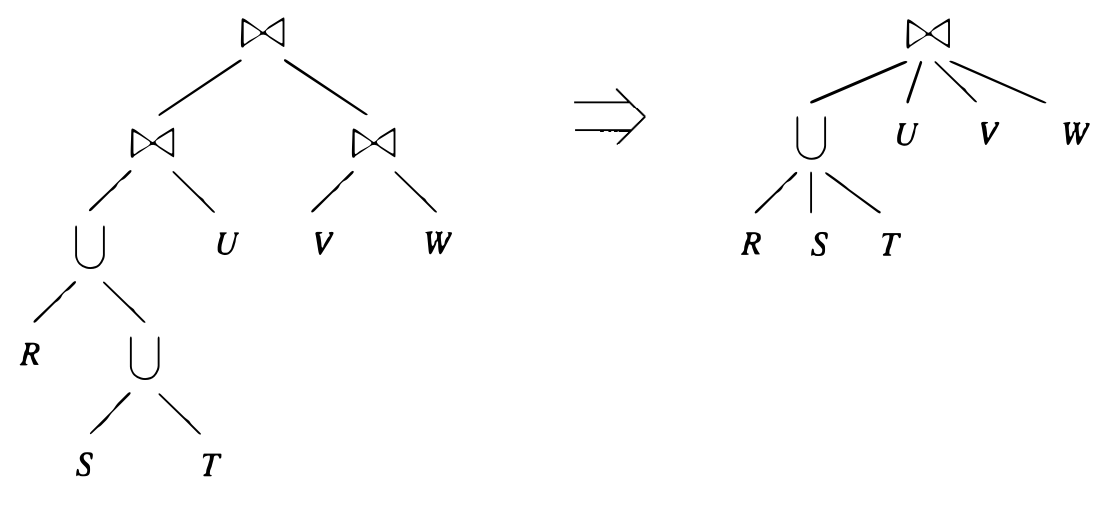
\includegraphics[scale=0.25]{multiple_children.png}\\
        \caption{An example associative operators being grouped}
        \label{fig:j_2}
    \end{figure}
\end{frame}

\begin{frame}{SQL: Cost Estimation}
    a
\end{frame}

\begin{frame}{SQL}
    a
\end{frame}

\begin{frame}{SQL}
    a
\end{frame}

\begin{frame}{SQL}
    a
\end{frame}


\begin{frame}{Data Streams}
    Stream query optimization is the process of modifying a stream processing query, often by changing  its  graph  topology  and or  operators,  with the  aim  of  achieving  better  performance  (such as  higher  throughput,  lower  latency,  or  reduced resource usage), while preserving the semantics of the original query.\\
    Stream  query  optimizations  are  best  understood  with  respect  to  stream  graphs.  A stream graph is a directed graph whose edges are streams and  whose  nodes  are  operators.  Root  and  leaf nodes are called sources and sinks, respectively.
\end{frame}

\begin{frame}{Possible Optimizations}
    \begin{itemize}
        \item Batching
        \item Placement
        \item State sharing
        \item Load Balancing
        \item Algorithm selection
        \item Load Shedding
        \item Fusion
        \item Operator Separation
        \item Operator Reordering
        \item Redundancy elimination
        \item Fission
    \end{itemize}
    We focus on Operator Reordering.
\end{frame}

\begin{frame}{Deep Neural Networks}
    To understand a neural network we should first look at a neuron. 
    \begin{figure}
        \centering
        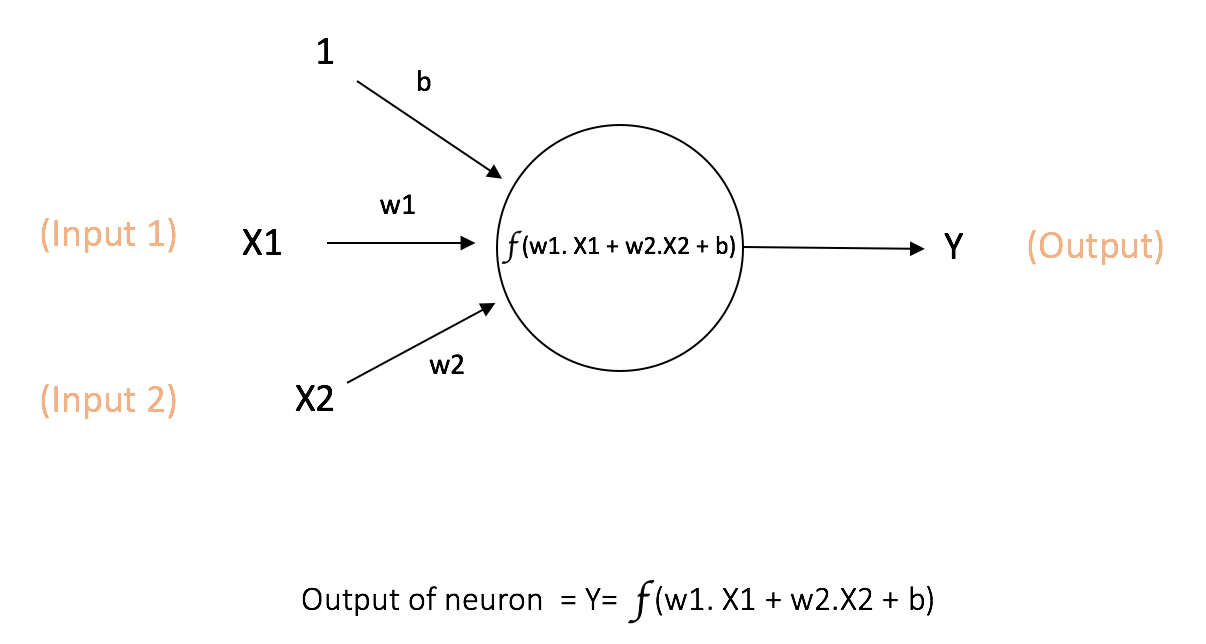
\includegraphics[scale=0.5]{neuron.png}\\
        \caption{Example of a neuron}
        \label{fig:neuron}
    \end{figure}
    $f$ is generally taken to be a non linear function. This non linearity grants neural networks additional flexibility.
\end{frame}


\begin{frame}{Deep Neural Networks}
    Deep neural networks is a layer wise combinations of neurons\\
    Building up on the neuron seen in the last slide. We have
    \begin{figure}
        \centering
        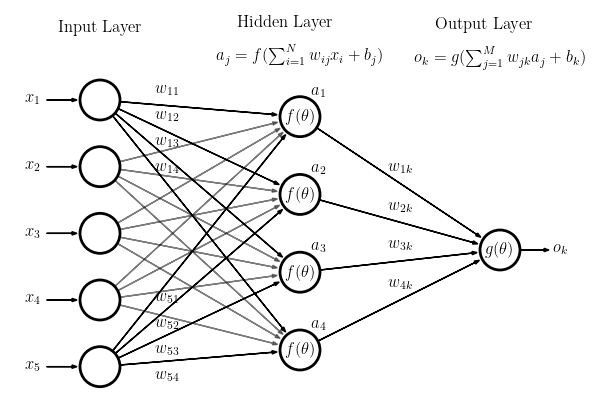
\includegraphics[scale=0.5]{dl.png}\\
        \caption{Example of a deep neural network}
        \label{fig:dl}
    \end{figure}
\end{frame}

\begin{frame}{Backpropogation}
    How does a neural network train on these parameters? First look at how a single node back propogates.
    \begin{figure}
        \centering
        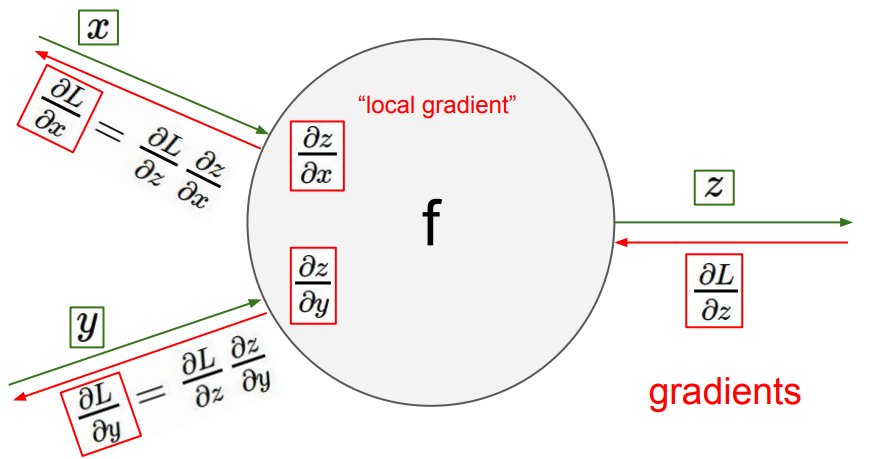
\includegraphics[scale=0.25]{nbp.png}\\
        \caption{Example of backpropogation on a node}
        \label{fig:nbp}
    \end{figure}
\end{frame}

\begin{frame}{Backpropogation}
    By doing backpropogation on each node, we finish the process. 
    \begin{figure}
        \centering
        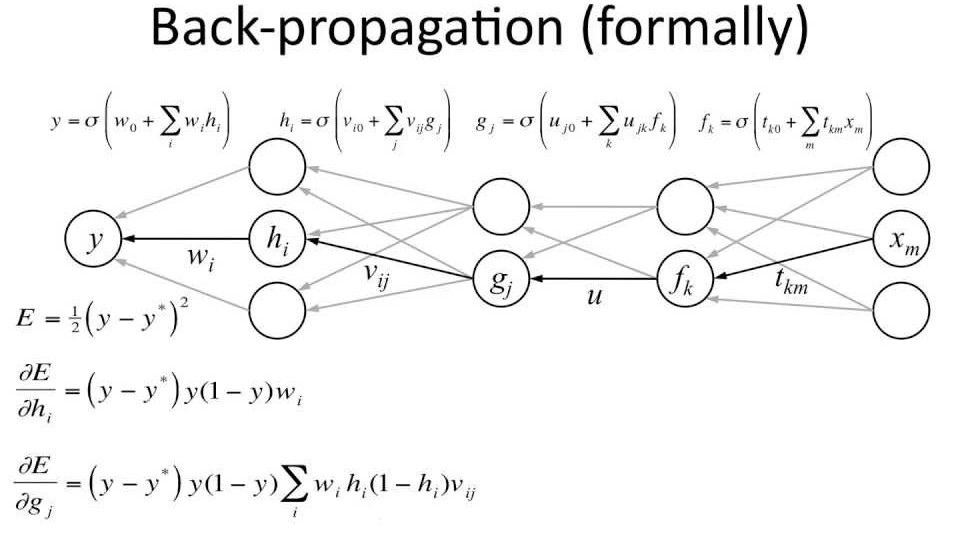
\includegraphics[scale=0.25]{bp.jpg}\\
        \caption{Example of backpropogation }
        \label{fig:bp}
    \end{figure}
\end{frame}

\begin{frame}{Reinforcement Learning}
    What is reinforcement learning? How is it different from supervised and unsupervised learning?
    \begin{figure}
        \centering
        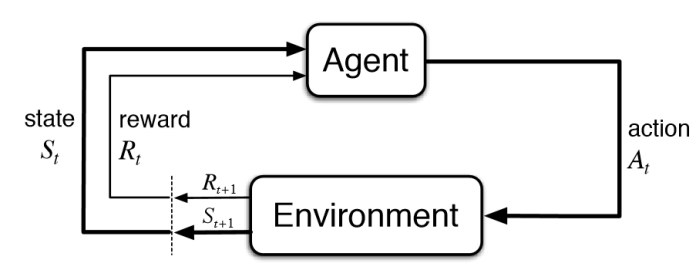
\includegraphics[scale=0.5]{rl.jpg}\\
        \caption{Example of a framework of a reinforcement learning agent }
        \label{fig:rl}
    \end{figure}
\end{frame}

\begin{frame}[fragile]{Value Iteration}
    \begin{lstlisting}[language=python, caption=value iteration algorithm]
    for s in S:
        V(s)=0
    while(not converged):
        for s in S:
            V(s)=R(s)+max over all action[gamma*(sum(P(s,a,s')V(s')))]
    \end{lstlisting}
\end{frame}

\begin{frame}[fragile]{Policy Iteration}
\begin{lstlisting}[language=python, caption=Policy iteration algorithm]
initialize random pi
while(not converged):
    V=V(pi)
    for s in S:
        pi(s)=max over all actions[sum(P(s,a,s')V(S'))]
\end{lstlisting}
\end{frame}

\begin{frame}{Deep Reinforcement Learning}
    Deep reinforcement learning combines Deep learning and reinforcement learning
    \begin{figure}
        \centering
        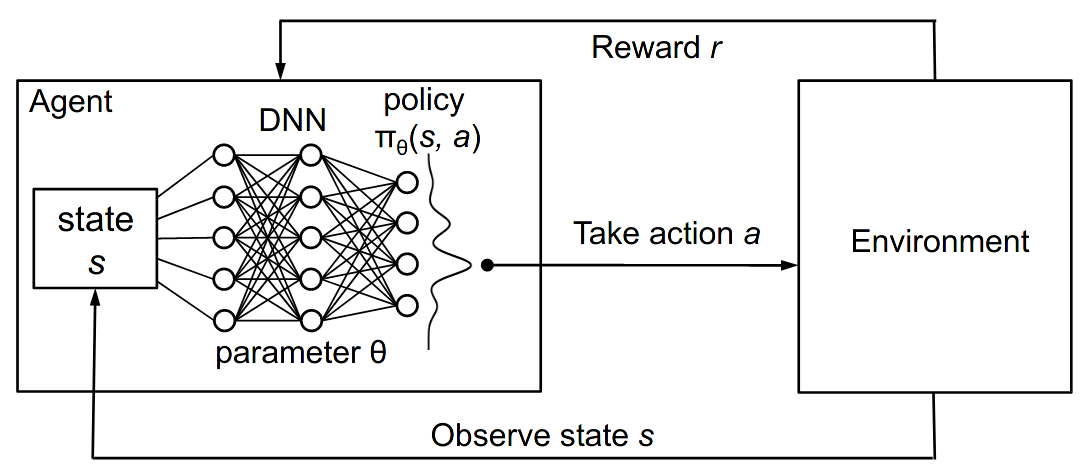
\includegraphics[scale=0.25]{drl.png}\\
        \caption{Deep Reinforcement learning(DQN) framework}
        \label{fig:drl}
    \end{figure}
\end{frame}
